\section{Prinsip Induksi Matematika}

\logic{Induksi matematika} adalah teknik pembuktian fundamental untuk membuktikan bahwa suatu pernyataan $P(n)$ benar untuk semua bilangan bulat $n$ di atas nilai awal tertentu \cite{levin_discrete,brilliant_induction,rosen2019}. Teknik ini sangat penting dalam matematika diskret dan ilmu komputer karena banyak struktur diskret---seperti barisan, graf, dan algoritma rekursif---dapat dianalisis dengan induksi. Analogi domino sering dipakai untuk menggambarkan prinsip ini: jika domino pertama jatuh dan setiap domino yang jatuh menyebabkan domino berikutnya jatuh, maka seluruh barisan domino akan jatuh \cite{brilliant_induction,discrete_induction}.

Prinsip formal induksi matematika, sering disebut PMI (Principle of Mathematical Induction), terdiri atas dua langkah \cite{discrete_induction,wiki_induction}. Pertama, buktikan kasus basis: $P(n_0)$ benar untuk bilangan awal $n_0$ (biasanya $n_0 = 0$ atau $n_0 = 1$). Kedua, buktikan langkah induktif: untuk sembarang $k \geq n_0$, jika $P(k)$ benar (hipotesis induksi), maka $P(k+1)$ benar. Jika kedua langkah berhasil dibuktikan, kita dapat menyimpulkan bahwa $P(n)$ benar untuk semua $n \geq n_0$ \cite{levin_discrete,uottawa_induction}.

Kasus basis tidak boleh diabaikan \cite{brilliant_induction,libretexts_induction}. Memverifikasi $P(n_0)$ secara eksplisit sangat penting karena tanpa basis yang valid, langkah induktif saja tidak menjamin kebenaran pernyataan. Terdapat contoh bukti induksi yang keliru karena basis salah atau tidak diverifikasi, sehingga menghasilkan kesimpulan palsu. Oleh karena itu, selalu pastikan basis diverifikasi dengan teliti sebelum melanjutkan ke langkah induktif \cite{discrete_induction,rosen2019}.

Hipotesis induksi adalah asumsi bahwa $P(k)$ benar untuk suatu $k$ sembarang \cite{uottawa_induction,mit_6042}. Asumsi ini bukan mengambil kesimpulan begitu saja, melainkan diasumsikan sementara untuk menunjukkan implikasi $P(k) \Rightarrow P(k+1)$. Karena $k$ sembarang, jika kita telah membuktikan basis $P(n_0)$ dan implikasi tersebut, maka $P(n_0) \Rightarrow P(n_0+1) \Rightarrow P(n_0+2) \Rightarrow \cdots$, sehingga $P(n)$ benar untuk semua $n \geq n_0$. Pola ini mencerminkan sifat well-ordering dari bilangan asli: setiap himpunan bilangan asli tak kosong memiliki elemen terkecil \cite{levin_discrete,wiki_induction}.

Secara ringkas, struktur bukti induksi standar selalu mengikuti pola yang sama: verifikasi basis, lalu buktikan langkah induktif dari $P(k)$ ke $P(k+1)$ \cite{brilliant_induction,libretexts_induction}. Format berikut memudahkan pembaca memahami alur bukti dan memastikan tidak ada langkah yang terlewat. Banyak buku teks dan sumber OER merekomendasikan mengikuti format standar ini, terutama bagi pemula \cite{discrete_induction,uwo_induction}.

Untuk membuktikan bahwa $P(n)$ benar untuk semua bilangan bulat $n \geq n_0$ \cite{levin_discrete,discrete_induction}:

\begin{enumerate}
  \item \textbf{Basis}: Buktikan $P(n_0)$ benar.
  \item \textbf{Langkah Induktif}: Asumsikan $P(k)$ benar (hipotesis induksi) untuk suatu $k \geq n_0$, lalu buktikan $P(k+1)$ benar.
\end{enumerate}

Gambar~\ref{fig:alur-induksi} mengilustrasikan alur bukti induksi dari basis menuju kesimpulan \cite{discrete_induction,brilliant_induction}.

\begin{figure}[htbp]
\centering
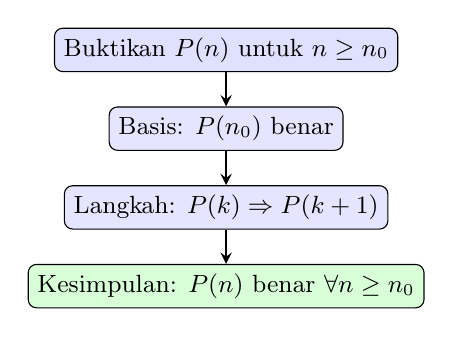
\begin{tikzpicture}[node distance=0.9cm, font=\small, box/.style={rectangle, draw=black, rounded corners=3pt, minimum width=2.8cm, align=center, fill=#1}]
  \node[box=blue!12] (b1) at (0,2) {Buktikan $P(n)$ untuk $n \geq n_0$};
  \node[box=blue!10] (b2) at (0,1) {Basis: $P(n_0)$ benar};
  \node[box=blue!10] (b3) at (0,0) {Langkah: $P(k) \Rightarrow P(k+1)$};
  \node[box=green!15] (b4) at (0,-1) {Kesimpulan: $P(n)$ benar $\forall n \geq n_0$};
  \draw[thick, ->, >=stealth] (b1) -- (b2);
  \draw[thick, ->, >=stealth] (b2) -- (b3);
  \draw[thick, ->, >=stealth] (b3) -- (b4);
\end{tikzpicture}
\caption{Alur bukti induksi matematika: basis, langkah induktif, dan kesimpulan}
\label{fig:alur-induksi}
\end{figure}

Tabel~\ref{tab:struktur-induksi} merangkum langkah-langkah dan verifikasi yang diperlukan \cite{levin_discrete,rosen2019}.

\begin{table}[htbp]
\centering
\small
\begin{tabular}{|>{\raggedright\arraybackslash}p{2.2cm}|>{\raggedright\arraybackslash}p{4.2cm}|>{\raggedright\arraybackslash}p{4.2cm}|}
\hline
\textbf{Langkah} & \textbf{Deskripsi} & \textbf{Verifikasi} \\
\hline
Basis & Buktikan $P(n_0)$ benar & Hitung/cek $P(n_0)$ secara eksplisit \\
\hline
Hipotesis induksi & Asumsikan $P(k)$ benar untuk suatu $k \geq n_0$ & Asumsi, tidak dibuktikan di langkah ini \\
\hline
Langkah induktif & Turunkan $P(k+1)$ dari $P(k)$ & Manipulasi aljabar atau logika dari $P(k)$ \\
\hline
Kesimpulan & $P(n)$ benar untuk semua $n \geq n_0$ & Berdasarkan prinsip induksi \\
\hline
\end{tabular}
\caption{Struktur bukti induksi: langkah dan verifikasi}
\label{tab:struktur-induksi}
\end{table}

Untuk pernyataan $P(n): 1 + 2 + \cdots + n = n(n+1)/2$, Tabel~\ref{tab:nilai-Pn} memverifikasi beberapa nilai awal (bukan pengganti bukti, melainkan ilustrasi).

\begin{table}[htbp]
\centering
\small
\begin{tabular}{|c|c|c|c|}
\hline
\textbf{$n$} & \textbf{LHS $(1+\cdots+n)$} & \textbf{RHS $n(n+1)/2$} & \textbf{Cocok?} \\
\hline
1 & 1 & 1 & Ya \\
\hline
2 & 3 & 3 & Ya \\
\hline
3 & 6 & 6 & Ya \\
\hline
4 & 10 & 10 & Ya \\
\hline
\end{tabular}
\caption{Contoh nilai $P(n)$ untuk $1+2+\cdots+n = n(n+1)/2$}
\label{tab:nilai-Pn}
\end{table}

\begin{contoh}
Buktikan $1 + 2 + \cdots + n = \frac{n(n+1)}{2}$ untuk $n \geq 1$ \cite{levin_discrete,brilliant_induction}.

Basis: Untuk $n=1$, ruas kiri (LHS) sama dengan $1$, dan ruas kanan (RHS) sama dengan $1(2)/2 = 1$. Jadi $P(1)$ benar.

Langkah induktif: Asumsikan $1+\cdots+k = k(k+1)/2$ untuk suatu $k \geq 1$ (hipotesis induksi). Maka
\begin{align*}
1+\cdots+k+(k+1)
  &= \frac{k(k+1)}{2} + (k+1)
  = (k+1)\left(\frac{k}{2}+1\right)\\
  &= \frac{(k+1)(k+2)}{2}
  = \frac{(k+1)\big((k+1)+1\big)}{2}.
\end{align*}
Ini menunjukkan bahwa $P(k+1)$ benar. Berdasarkan prinsip induksi matematika, $1 + 2 + \cdots + n = n(n+1)/2$ benar untuk semua $n \geq 1$.
\end{contoh}

Analogi domino (Gambar~\ref{fig:domino-induksi}): jika domino pertama jatuh dan setiap domino yang jatuh menjatuhkan domino berikutnya, maka seluruh barisan jatuh \cite{brilliant_induction}.

\begin{figure}[htbp]
\centering
\begin{tikzpicture}[node distance=0.4cm, font=\small, domino/.style={rectangle, draw=black, fill=blue!15, minimum width=0.7cm, minimum height=1.2cm}]
  \node[domino] (d1) at (0,0) {};
  \node[domino] (d2) at (1.2,0) {};
  \node[domino] (d3) at (2.4,0) {};
  \node[domino] (d4) at (3.6,0) {};
  \draw[thick, ->, >=stealth] (0.45,0) -- (0.75,0);
  \draw[thick, ->, >=stealth] (1.65,0) -- (1.95,0);
  \draw[thick, ->, >=stealth] (2.85,0) -- (3.15,0);
  \node[below=0.1cm of d2] {\scriptsize $P(n_0)$};
  \node[below=0.1cm of d3] {\scriptsize $P(k)\!\Rightarrow\!P(k{+}1)$};
\end{tikzpicture}
\caption{Analogi domino: basis (domino pertama jatuh) dan langkah induktif (setiap domino menjatuhkan berikutnya)}
\label{fig:domino-induksi}
\end{figure}

\begin{contoh}
Buktikan $2^n > n$ untuk $n \geq 1$ \cite{levin_discrete,rosen2019}.

Basis: Untuk $n=1$, $2^1 = 2 > 1$, jadi $P(1)$ benar.

Langkah induktif: Asumsikan $2^k > k$ untuk suatu $k \geq 1$. Maka $2^{k+1} = 2 \cdot 2^k > 2k \geq k+1$ (karena $k \geq 1$ maka $2k \geq k+1$). Jadi $P(k+1)$ benar. Berdasarkan induksi, $2^n > n$ untuk semua $n \geq 1$.
\end{contoh}

\subsection*{Verifikasi numerik}

Verifikasi numerik dengan program bukan pengganti bukti induksi, tetapi dapat memperkuat pemahaman dan memeriksa rumus untuk banyak nilai \cite{levin_discrete}. Gambar~\ref{fig:verifikasi-jumlah} membandingkan $S_n = 1+2+\cdots+n$ dengan rumus $n(n+1)/2$ untuk $n = 1, \ldots, 20$.

\begin{figure}[htbp]
\centering

\includegraphics[width=0.85\textwidth]{bab-07/verifikasi-jumlah-n}
\caption{Verifikasi numerik: $1+2+\cdots+n$ vs $n(n+1)/2$}
\label{fig:verifikasi-jumlah}
\end{figure}

Kode Python berikut memverifikasi rumus jumlah dan ketaksamaan $2^n > n$ untuk beberapa nilai $n$ \cite{python_docs_boolean}.

\begin{lstlisting}[style=pythonstyle, caption={Verifikasi numerik rumus $1+2+\cdots+n = n(n+1)/2$ dan $2^n > n$}]
# Verifikasi 1 + 2 + ... + n = n(n+1)/2
for n in range(1, 21):
    lhs = sum(range(1, n + 1))
    rhs = n * (n + 1) // 2
    assert lhs == rhs, f"n={n}: {lhs} != {rhs}"
print("Rumus 1+2+...+n = n(n+1)/2 OK untuk n=1..20")

# Verifikasi 2^n > n untuk n >= 1
for n in range(1, 21):
    assert 2**n > n, f"2^{n} > {n} gagal"
print("Ketaksamaan 2^n > n OK untuk n=1..20")
\end{lstlisting}

\begin{konsep}
Induksi matematika: (1) Basis---buktikan $P(n_0)$; (2) Langkah induktif---buktikan $P(k) \Rightarrow P(k+1)$ untuk $k \geq n_0$. Jika keduanya terbukti, $P(n)$ benar untuk semua $n \geq n_0$. Jangan lupa verifikasi basis; hipotesis induksi adalah asumsi, bukan kesimpulan.
\end{konsep}
